\chapter[The present AWAKE eBPM system]{The present AWAKE eBPM system}

AWAKE uses a copropagating electron and proton beam. The proton beam has a repetition rate of 10 Hz, while the proton beam from the SPS comes with time intervals in the order of the minute(s).

The simultaneous, shot-by-shot, measurement of the position of the electron and proton beams is desirable. All the experiments so far conduced assuming that the electron position did not drift in the shot with protons. The presence of protons blinds the present electron diagnostic.

\section[Equipment description]{Equipment description}

\subsection[Beamline and diagnostic]{Beamline and diagnostic}

Description of the SPS beamline, of the electron beamline and general other instrumentation installed (including the proton BPMs).

\subsection[Electron BPMs]{Electron BPMs}

The electron beam position monitoring system of the AWAKE facility was developed at TRIUMF\footnote{TRIUMF, Canada's Particle Accelerator Centre, Vancouver, BC, Canada, \url{https://www.triumf.ca/}}. It is composed by shorted stripline-type beam position monitor, and the readout electronics in charge of the signal processing.

\subsubsection{Beam position monitor}

Two types of beam position monitors are installed in the beamlines. In the electron beamline 40 mm aperture BPMs are used, while in the common beamline the 60 mm aperture model is used. The working principle is the same and they differ mostly on the mechanical dimensions. The coverage angle is 38 degrees, with a longitudinal lenght of 120 and 124 mm, respectively.

\subsubsection{Readout electronics}

GENERALITIES ON THE ELECTRONICS


\section[Beam spectrum]{Beam spectrum}

Intro to section.

\subsection[Gaussian beams]{Gaussian beams}

\subsection[Real beams]{Real beams}


\section[Measurements with beam]{Measurements with beam}

A number of measurements performed on BPM51 with and without beam

\subsection[Electrode signals]{Electrode signals}

with and without proton beam

\subsection[VNA measurements]{VNA measurements}

40 and 60 mm type

\section[Electromagnetic simulations]{Electromagnetic simulations}

A 3D parametric model was created in CST STUDIO SUITE\textregistered~2018 on the basis of the drawings provided by TRIUMF. The comparison between the CST model and the drawings is shown in Fig.~\ref{CSTvsSTEP}~and~\ref{CSTvsSTEP_section}. It is important to note that none of the vacuum feedthrough was modeled in CST, as it is inaccurately reported also in the technical drawings as it constitutes industrial secret. In the simulations the signal is collected from the striplines through waveguide ports placed at the end of coaxial lines. The central cilindrical pin of the coaxial line is retained at the design value, while the surrounding vacuum diameter was selected in order to match the line impedance to $50\,\Omega$, in order to avoid unwanted reflections.

The beam position monitor geometry is transversely symmetric. Whenever possible, this has been used to reduce the computing time, imposing boundary conditions.

The simulations regarded mostly calculating the signal response to the beam excitation with different bunch lenghts and the full characterisation of the device as a four port network, calculating the scattering parameters. The former is realised via wakefield simulations, and the latter via frequency domain simulations.

\begin{figure}[t]
\centering
\subfigure[CST model]
  {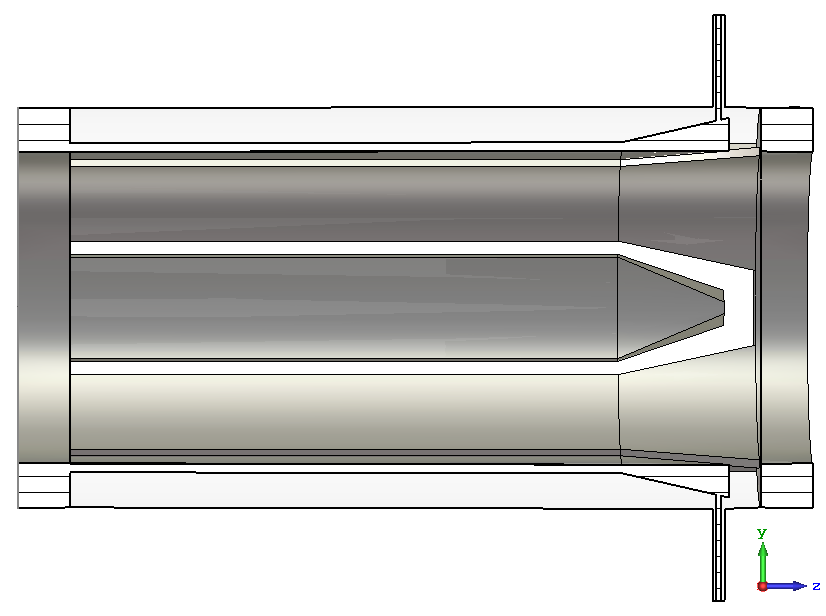
\includegraphics[width=6.5cm,height=5cm]{pictures/CST_section}}
\hspace{3mm}
\subfigure[TRIUMF mechanical model]
  {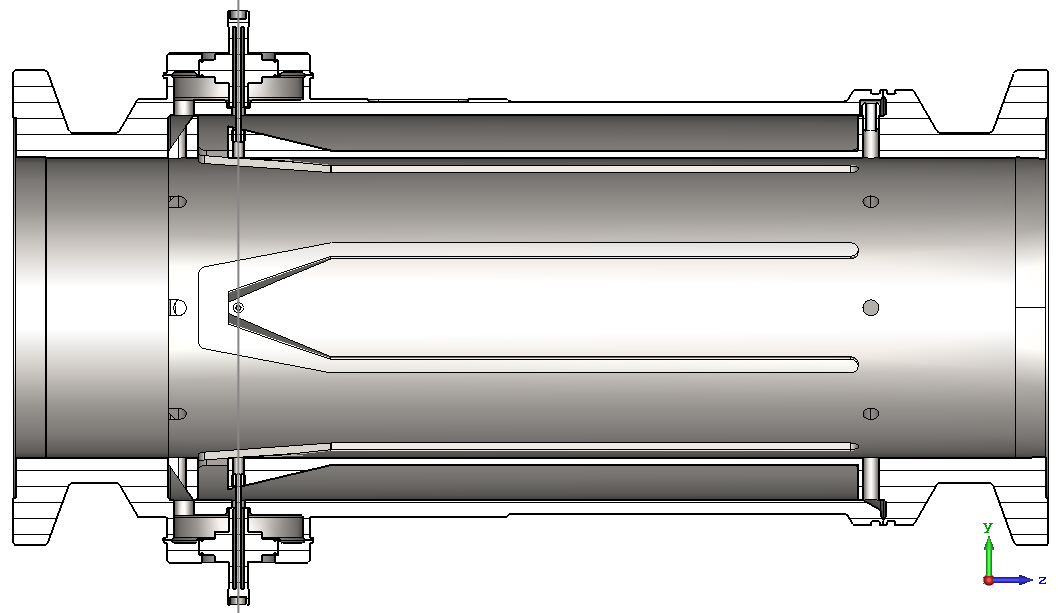
\includegraphics[width=6.5cm,height=5cm]{pictures/STEP_section}}
\caption{3D models used in the electromagnetic simulations (a) and the original mechanical design (b). }
\label{CSTvsSTEP_section}
\end{figure}



\subsection[Electrode signals]{Electrode signals}

WAK sims

\subsection[Four-port device characterisation in simulations]{Four-port device characterisation in simulations}

Sparam sims





\section[Optimisations]{Optimisations}

\subsection[Impedance matching of the stripline termination]{Impedance matching of the stripline termination}

TDR studies showed that the impendance matching to 50~$\Omega$ of the striplines is not sufficiently optimised. In the attempt of understanding if this could be the source of the resonant response of the device, an geomterical optimisation of the tapered part of the stripline has been carried out. This is realised via parametric time domain simulations, observing the variation of the TDR response. Successively, a wakefield simulation was carried out with the improved geometry, comparing the electrode signal to the unoptimised version.

Something something ...

Mention that in the development phase, this geometry was optimised using the ANSYS\textregistered~HFSS\texttrademark~electromagnetic simulation code\footnote{\url{https://www.ansys.com/products/electronics/ansys-hfss}}, but it had to be modified due to manufacturing constraints during the mechanical design phase\cite{Victor:private-comm}


\subsection[Geometrical optimisation of the space behind the stripline]{Geometrical optimisation of the space behind the stripline}

Same process, but for the
